\documentclass[25pt]{beamer}
\usecolortheme[dark]{solarized/beamercolorthemesolarizedUniPD}

\usepackage[utf8]{inputenc}
\usepackage[english]{babel}
\usepackage[absolute,overlay]{textpos}
\usepackage{listings}
\usepackage{color}
\usepackage{siunitx}


\definecolor{mygreen}{rgb}{0,0.6,0}
\definecolor{mygray}{rgb}{0.5,0.5,0.5}
\definecolor{mymauve}{rgb}{0.58,0,0.82}

\lstset{ %
  basicstyle=\footnotesize,        % the size of the fonts that are used for the code
  breakatwhitespace=false,         % sets if automatic breaks should only happen at whitespace
  breaklines=true,                 % sets automatic line breaking
  captionpos=b,                    % sets the caption-position to bottom
  commentstyle=\color{mygreen},    % comment style
  deletekeywords={...},            % if you want to delete keywords from the given language
  escapeinside={\%*}{*)},          % if you want to add LaTeX within your code
  extendedchars=true,              % lets you use non-ASCII characters; for 8-bits encodings only, does not work with UTF-8
  frame=single,                    % adds a frame around the code
  keepspaces=true,                 % keeps spaces in text, useful for keeping indentation of code (possibly needs columns=flexible)
  keywordstyle=\color{blue},       % keyword style
  language=Octave,                 % the language of the code
  morekeywords={*,...},            % if you want to add more keywords to the set
  numbers=left,                    % where to put the line-numbers; possible values are (none, left, right)
  numbersep=5pt,                   % how far the line-numbers are from the code
  numberstyle=\tiny\color{mygray}, % the style that is used for the line-numbers
  rulecolor=\color{mygray},         % if not set, the frame-color may be changed on line-breaks within not-black text (e.g. comments (green here))
  showspaces=false,                % show spaces everywhere adding particular underscores; it overrides 'showstringspaces'
  showstringspaces=false,          % underline spaces within strings only
  showtabs=false,                  % show tabs within strings adding particular underscores
  stepnumber=2,                    % the step between two line-numbers. If it's 1, each line will be numbered
  stringstyle=\color{orange},     % string literal style
  tabsize=2,                       % sets default tabsize to 2 spaces
  title=\lstname                   % show the filename of files included with \lstinputlisting; also try caption instead of title
}

\lstdefinelanguage{XML}
{
  morestring=[b]",
  morestring=[s]{>}{<},
  morecomment=[s]{<?}{?>},
  identifierstyle=\color{cyan},
  keywordstyle=\color{purple},
  morekeywords={xmlns,version,type}% list your attributes here
}


\title{On Lightweight Mobile Phone Application Certification\\}
\subtitle{\textit{\small{William Enck, Machigar Ongtang and Patrick McDaniel\\The Pennsylvania State University}}}
\author{Marco Zanella}
\date{10th January 2018}
\institute{Computer and Network Security}

\begin{document}
\graphicspath{{res/img/}}

\newcommand{\turnOffNumbers}{true}

\fontsize{18pt}{7.2}\selectfont

\begin{frame}[plain,noframenumbering]
  \titlepage
\end{frame}

\let\turnOffNumbers\empty

\begin{frame}[fragile]{Android background}
  \begin{center}
  \begin{itemize}
    \item Components
    \begin{itemize}
      \item <2-> Activity
      \item <3-> Service
      \item <4-> Content Provider
      \item <5-> Broadcast Receiver
      \item <6-> Intent
    \end{itemize}
    \vfill
    \item Permission labels \\ 

\onslide<7-> 
\begin{lstlisting}[language=XML]
<uses-permission android:name="android.permission.INTERNET"/>
\end{lstlisting}

  \begin{textblock*}{1cm}(8.5cm, 2.5cm)
    
\includegraphics[scale=0.3]{androidwhite}
  \end{textblock*}


  \end{itemize}
  \end{center}
\end{frame}
\begin{frame}[fragile]{Permission levels}
  4 levels
  \begin{center}
  \begin{enumerate}
    \item ``normal''\\
    granted to any app that requires it

    \vspace*{0.4cm}

    \item ``dangerous''\\
    requires user confirmation

    \vspace*{0.4cm}

    \item ``signature''\\
    app must be signed with a developer key

    \vspace*{0.4cm}

    \item ``signature or system''\\
    compatibility with older system
  \end{enumerate}

  \begin{textblock*}{1cm}(10cm, 3.6cm)
    
\includegraphics[scale=0.14]{levels}
  \end{textblock*}

  \end{center}
\end{frame}
\begin{frame}[fragile]{Smartphone security}
  
  Smartphone has lots of sensitive data so there are lots of possible attacks

  \vfill
  
  Android permission label system is based on the user capacity

  \vfill

  Apple (and Symbian) inspect source code in order to prevent software misuse
  and malware propagation but it is really expansive

\end{frame}

\begin{frame}{Kirin - 1}

What is Kirin
\begin{center}
  \begin{itemize}
    \item It is a lightweight certification at install time

    \vfill

    \item Rules that must be followed by the application in order to allow the
    installation

    \vfill

    \item It includes a language for the rule definition
  \end{itemize}
\end{center}

\begin{textblock*}{1cm}(9cm, 7.2cm)
    
\includegraphics[scale=0.25]{kirin}
\end{textblock*}

\end{frame}
\begin{frame}{Kirin - 2}

\begin{figure}
  \centering
  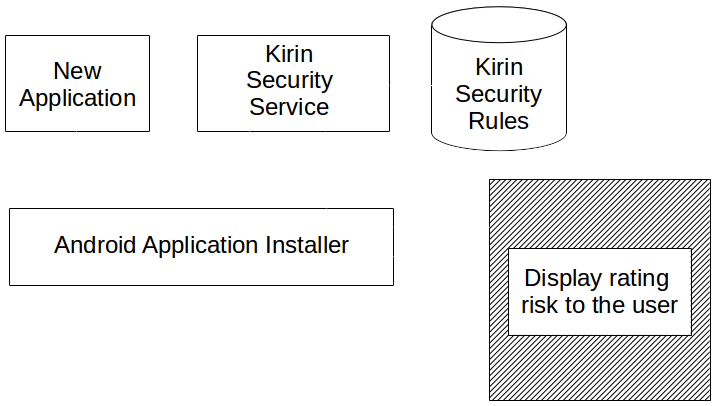
\includegraphics[scale=0.55]{kirinscheme}
\end{figure}

\end{frame}
\begin{frame}{Kirin rules defining process}

\begin{figure}
  \centering
  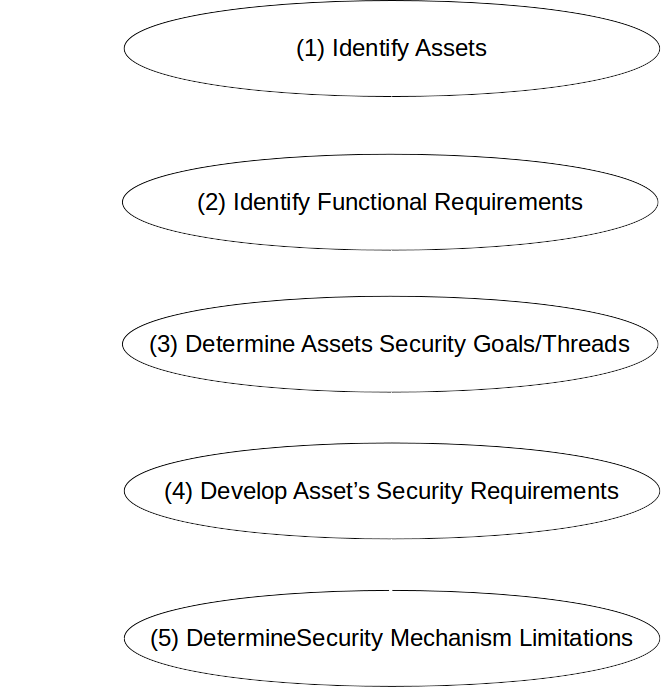
\includegraphics[scale=0.34]{ruleprocess}
\end{figure}

\end{frame}
\begin{frame}{Example of a set of rules}
\vspace*{-0.4cm}

\fontsize{9pt}{0}\selectfont
  (1) \textit{An application must not have the} \texttt{SET\_DEBUG\_APP}
  \textit{permission label.}\\ \vspace*{0.2cm}
  (2) \textit{An application must not have} \texttt{PHONE\_STATE},
  \texttt{RECORD\_AUDIO}\textit{, and }\texttt{INTERNET} \textit{permission
  labels.}\\ \vspace*{0.2cm}
  (3) \textit{An application must not have} \texttt{PROCESS\_OUTGOING\_CALL},
  \texttt{RECORD\_AUDIO}\textit{, and }\texttt{INTERNET} \textit{permission
  labels.}\\ \vspace*{0.2cm}
  (4) \textit{An application must not have} \texttt{ACCESS\_FINE\_LOCATION},
  \texttt{INTERNET}\textit{, and} \texttt{RECEIVE\_BOOT\_COMPLETE}
  \textit{permission labels.}\\ \vspace*{0.2cm}
  (5) \textit{An application must not have} \texttt{ACCESS\_COARSE\_LOCATION},
  \texttt{INTERNET}\textit{, and} \texttt{RECEIVE\_BOOT\_COMPLETE}
  \textit{permission labels.}\\ \vspace*{0.2cm}
  (6) \textit{An application must not have} \texttt{RECEIVE\_SMS} \textit{and}
  \texttt{WRITE\_SMS} \textit{permission labels.}\\ \vspace*{0.2cm}
  (7) \textit{An application must not have} \texttt{SEND\_SMS} \textit{and}
  \texttt{WRITE\_SMS} \textit{permission labels.}\\ \vspace*{0.2cm}
  (8) \textit{An application must not have} \texttt{INSTALL\_SHORTCUT}
  \textit{and} \texttt{UNINSTALL\_SHORTCUT} \textit{permission labels.}
  \\ \vspace*{0.2cm}
  (9) \textit{An application must not have the}
  \texttt{SET\_PREFERRED\_APPLICATION} \textit{permission label and receive
  Intents for the} \texttt{CALL} \textit{action string.}\\ \vspace*{0.2cm}
\fontsize{25pt}{7.2}\selectfont

\end{frame}


\begin{frame}{Evaluation - $1^{st}$ run}

\begin{center}
  \begin{itemize}
    \item Tested Kirin on 311

    \vfill

    \item 12 apps failed the test
    \begin{itemize}
    \item 3 apps failed \textbf{rule 2}

    \item 1 app failed \textbf{rule 4}

    \item 8 apps failed \textbf{rule 4 and 5}
    \end{itemize}
  \end{itemize}
\end{center}

\begin{textblock*}{1cm}(8cm, 1.8cm)
    
\includegraphics[scale=0.09]{test1}
\end{textblock*}

\begin{textblock*}{1cm}(9.5cm, 4.8cm)
    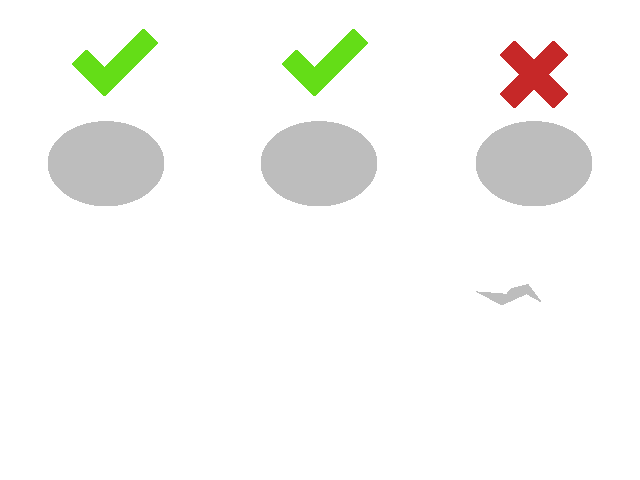
\includegraphics[scale=0.12]{test2}
\end{textblock*}

\begin{textblock*}{1cm}(7cm, 6.5cm)
    
\includegraphics[scale=0.05]{test3}
\end{textblock*}

\end{frame}

\begin{frame}{$1^{st}$ run - Failed rule 2}

\fontsize{10pt}{0}\selectfont
\begin{table}[]
\centering
\begin{tabular}{ll}
\textbf{App}              & \textbf{Description}                    \\[5pt] 
\hline\\[5pt]
Walkie Talkie Push to Talk & Walkie-Talkie style voice communication \\[5pt]
Shazam                    & Utility to identify music tracks        \\[5pt]
Inauguration Report       & Collaborative journalism application    \\[5pt]
\hline
\end{tabular}
\end{table}
\fontsize{15pt}{0}\selectfont

\vfill

\textbf{Rule 2} was create in order to avoid eavesdropper but none of these apps
have eavesdropper-like characteristics

\end{frame}

\begin{frame}{Rule 2 failure and changes}

\vspace*{-0.5cm}

\fontsize{13pt}{0}\selectfont

(2) \textit{An application must not have} \texttt{PHONE\_STATE},
\texttt{RECORD\_AUDIO}\textit{, and }\texttt{INTERNET} \textit{permission
labels.}\\

\vspace*{0.5cm}

Splitted into 2 sub-rules:\\
\hspace*{0.1cm}(2.1) add a \textbf{restriction} on receiving the 
\texttt{PHONE\_STATE} \hspace*{1.1cm}permission label\\
\hspace*{0.1cm}(2.2) add \texttt{RECEIVE\_BOOT\_COMPLETE} permission label

\vspace*{0.8cm}

With this change
\begin{itemize}
  \item 1 app failed \textbf{rule 2.1} and \textbf{rule 2.2} 
  (Walkie Talkie)

  \item 1 app failed \textbf{rule 4}

  \item 8 apps failed \textbf{rule 4 and 5}
\end{itemize}

\end{frame}
\begin{frame}{Failed rules 4 and 5}

\fontsize{10pt}{0}\selectfont
\begin{table}[]
\centering
\begin{tabular}{ll}
\textbf{App} & \textbf{Description} \\[5pt] \hline \\[5pt]
AccuTracking & Client for real-time GPS tracking service \\[8pt]
GPS Tracker* & Client for real-time GPS tracking service \\[8pt]
Loopt & \begin{tabular}[c]{@{}l@{}}Geosocial networking application
thatshares location \\[2pt] with friends\end{tabular} \\[13pt]
Twidroid & \begin{tabular}[c]{@{}l@{}}Twitter client that optionally allows
automatic\\[2pt] location tweets\end{tabular} \\[13pt]
Pintail & Reports the phone location in response toSMS message \\[8pt]
WeatherBug & Weather application with automaticweather alerts \\[8pt]
Homes & Classifieds application to aid in buyingor renting houses \\[8pt]
T-Mobile Hotspot & \begin{tabular}[c]{@{}l@{}}Utility to discover nearby nearby
T-Mobile WiFi \\[2pt] hotspots\end{tabular} \\[13pt]
Power Manager & \begin{tabular}[c]{@{}l@{}}Utility to automatically manage
radiosand \\[2pt] screen brightness\end{tabular}\\[5pt] \hline
\end{tabular}
\end{table}

\end{frame}
\begin{frame}{Kirin limitations}

\vspace*{-1cm}
\fontsize{15pt}{0}\selectfont
\begin{itemize}
  \item Limited expressiveness of Android policies

  \item Only checks manifest file

  \item Works only at installation time

  \item Not trivial to define rules
\end{itemize}

\vfill

\fontsize{18pt}{0}\selectfont
\begin{textblock*}{1cm}(2cm, 5.8cm)
  \includegraphics[scale=0.05]<2->{warning}
\end{textblock*}
\onslide<2->
\hspace*{3cm}
\textbf{Not a complete solution!}

\end{frame}
\begin{frame}{SAINT}

\fontsize{15pt}{0}\selectfont

\begin{itemize}
\item \textbf{S}ecure \textbf{A}pplication \textbf{INT}eraction

\vfill

\item Created with the goal to protect applications from other malicious
applications

\vfill

\item Developer defines policies in a similar way of permission labels

\vfill

\item Policies are enforced both at install and at run time
\end{itemize}

\begin{textblock*}{1cm}(9.8cm, 1.8cm)
    
\includegraphics[scale=0.25]{saint}
\end{textblock*}

\end{frame}
\begin{frame}{CR\^ePE}

\fontsize{15pt}{0}\selectfont

\vspace*{0.2cm}

\begin{itemize}
  \item \textbf{C}ontext-\textbf{Re}lated \textbf{P}olicy \textbf{E}nforcement

  \vfill

  \item Specify phone behaviour depending on the its current context

  \vfill

  \item Policy activated/deactivated depending on the context

  \vfill 

  \item Run-time permission changes with low overhead
\end{itemize}

\begin{textblock*}{1cm}(9.8cm, 1.6cm)
    
\includegraphics[scale=0.25]{cooking}
\end{textblock*}

\end{frame}
\begin{frame}{References}

\fontsize{9pt}{0}\selectfont

\begin{itemize}
  \item \textit{William Enck, Machigar Ongtang, and Patrick McDaniel}, 
  \textbf{On Lightweight Mobile Phone App Certification}, Proceedings of the
  16th ACM Conference on Computer and Communications Security (CCS), 2009.

  \vfill

  \item \textit{Machigar Ongtang, Stephen McLaughlin, William Enck, and Patrick
  McDaniel}, \textbf{Semantically Rich Application-Centric Security in Android},
  Proceedings of the 25th Annual Computer Security Applications Conference 
  (ACSAC), 2009.

  \vfill

  \item \textit{William Enck, Machigar Ongtang, and Patrick McDaniel},
  \textbf{Understanding Android Security}, IEEE Security \& Privacy Magazine,
  7(1):50--57, January/February, 2009.

  \vfill

  \item \textit{Mauro Conti, Bruno Crispo, Earlence Fernandes, Yury
  Zhauniarovich}, \textbf{CR\^ePE: a System for Enforcing Fine-Grained
  Context-Related Policies on Android}, IEEE Transactions on Information
  Forensics \& Security 2012.
\end{itemize}

\end{frame}

\end{document}
